\documentclass[a4paper,12pt]{article}
\usepackage{HomeWorkTemplate}
\usepackage{circuitikz}
\usepackage[shortlabels]{enumitem}
\usepackage{hyperref}
\usepackage{tikz}
\usepackage{amsmath}
\usepackage{amssymb}
\usepackage{tcolorbox}
\usepackage[normalem]{ulem} 
\usepackage{xepersian}
\settextfont{XB Niloofar}
\usetikzlibrary{arrows,automata}
\usetikzlibrary{circuits.logic.US}
\usepackage{changepage}
\newcounter{subproblemcounter}
\setcounter{subproblemcounter}{1}
\newcommand{\problem}[1]
{
	\subsection*{
		تمرین
		#1
	}
	\setcounter{subproblemcounter}{1}
}
\newcommand{\subproblem}{
	\textbf{\harfi{subproblemcounter})}\stepcounter{subproblemcounter}
}



\begin{document}
\handout
{طراحی پایگاه‌داده}
{دکتر مرتضی امینی}
{نیم‌سال اول 1401\lr{-}1402}
{اطلاعیه}
{امین کشیری، فاطمه توحیدیان، کسری حاجیان}
{۹۷۱۰۱۰۲۶, ۹۷۱۰۰۳۵۴, ۹۹۱۰۹۴۱۱}
 {فاز اول پروژه}


\section*{مفروضات و توضیحات: }
\begin{enumerate}
	\item در مدل طراحی شده هر مسافر دقیقا معادل یک بلیط در نظر گرفته شده‌است. با توجه به نیازمندی‌های 
	کنونی نیازی به مدل کردن مسافر نداشتیم. 
	\item از آنجایی که تنها گزینه‌ی موجود برای کلید خارجی زدن به موجودیت سوال، متن سوال بود، با توجه به حجم متن سوال تصمیم گرفتیم که صفت شناسه را به سوال اضافه کرده و آن را یک موجودیت قوی در نظر بگیریم. به دلیل مشابه موجودیت نظرسنجی نیز به یک موجودیت قوی تبدیل شد.
	\item گزارش یک نظرسنجی نیازی به مدل شدن ندارد. می‌توان آن  را به صورت یک صفت مشتق از 
	نظرسنجی در نظر گرفت. 
	\item با توجه به صورت نیازمندی‌ها، به نظر می‌رسد که 
	رابطه‌ی بین بلیط و نظرسنجی چند به چند است. یعنی این برداشت شده است که 
	با وجود این که یک بلیط یک بار در یک نظرسنجی می‌تواند شرکت کند،‌اما در نظرسنجی‌های 
	متفاوت آن شرکت می‌تواند شرکت کند. 
	\item در طراحی منطقی مدل سوال، تصمیم گرفتیم تنها از یک جدول استفاده کنیم 
	زیرا صفت اضافه‌ای نیاز نبود (کلید خارجی‌ها در مدل گزینه قرار می‌گرفتند).
	\item برای نمایش
	cardinality
	از روش 
	\lr{(min,max)}
	استفاده کردیم. 
	\item 
	فایل عکس 
	ERD 
	در کنار این 
	pdf 
	در فایل zip قرار گرفته‌است. 
\end{enumerate}


\section*{مدل‌سازی معنایی}

\begin{center}
	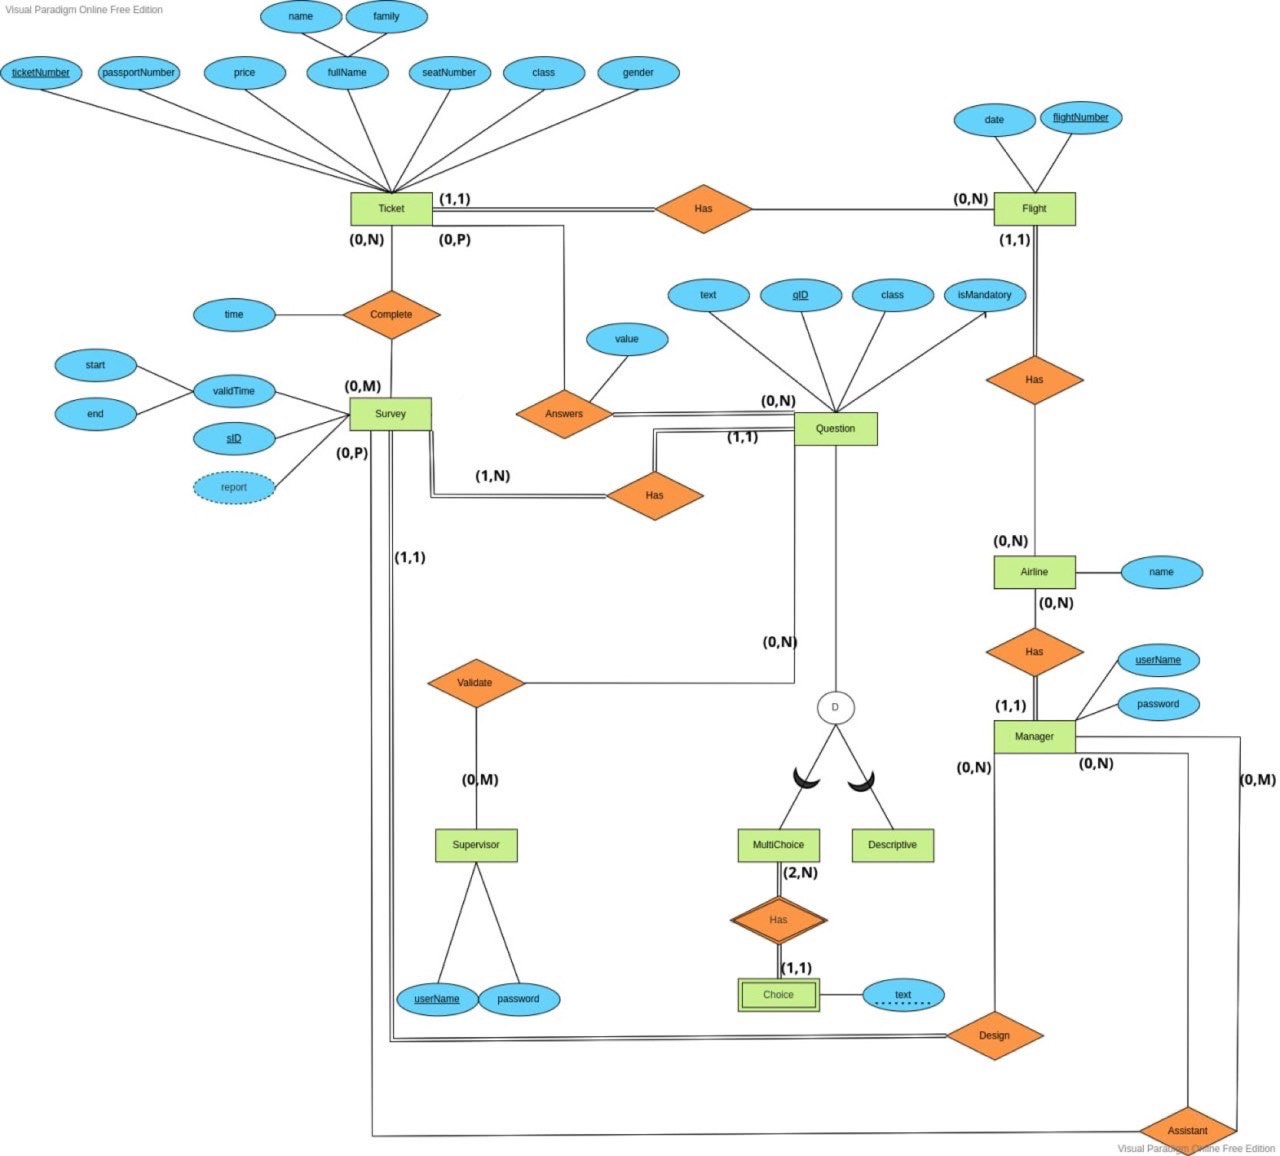
\includegraphics[scale=0.3]{ERD.png}
\end{center}

\section*{طراحی منطقی}

\begin{latin}
\

\textbf{Survey}(\underline{sID}, \dashuline{mUserName}, start, end)
\smallskip

\textbf{Airline}(\underline{name})
\smallskip

\textbf{Flight}(\underline{flightNumber}, \dashuline{airline}, date)
\smallskip

\textbf{Ticket}(\underline{ticketNumber}, name, family, passportNumber, \dashuline{flightNumber}, date, seatNumber, gender, price)
\smallskip

\textbf{Complete}(\underline{\dashuline{ticketNumber}, \dashuline{sID}}, time)
\smallskip

\textbf{Answers}(\dashuline{ticketNumber}, \dashuline{sID}, \dashuline{qID}, value)
\smallskip

\textbf{Question}(\underline{qID}, \dashuline{sID}, text, class, isMandatory, type)
\smallskip

\textbf{Choice}(\underline{\dashuline{qID}, text})
\smallskip

\textbf{Supervisor}(\underline{userName}, password)
\smallskip

\textbf{Validated}(\underline{\dashuline{qID}, \dashuline{sUserName}})
\smallskip

\textbf{Manager}(\underline{userName}, password, \dashuline{airline})
\smallskip

\textbf{Assistant}(\underline{\dashuline{mUserName}, \dashuline{aUserName}, \dashuline{sID}})
\smallskip

\end{latin}

\end{document}